\begin{enumerate}
    \item The synchronous sequential circuit shown below works at a clock frequency of $\qty{1}{\giga\hertz}$. The throughput, in $\SI{}{\mega\bit\per\second}$ and the latency, in $ns$, respectively, are 

\begin{figure}[ht]
    \centering
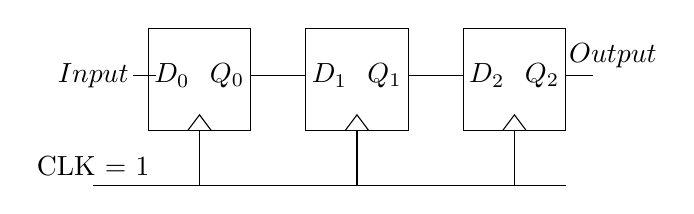
\begin{tikzpicture}
\ctikzset{                                   
    logic ports=ieee,                   
    logic ports/scale=0.5               
}                                    

% Drawing flip-flops
\draw (-1.3,-1.3) rectangle (0,0);
\draw(-1,-0.6) node{$D_0$};
\draw(-0.3,-0.6) node{$Q_0$};
\draw(0.7,-1.3) rectangle (2,0);
\draw(1,-0.6) node{$D_1$};
\draw(1.7,-0.6) node{$Q_1$};
\draw(2.7,-1.3) rectangle (4,0);
\draw(3,-0.6) node{$D_2$};
\draw(3.7,-0.6) node{$Q_2$};

% Connecting them
\draw(0,-0.6) -- (0.7,-0.6);
\draw(2,-0.6) -- (2.7,-0.6);
\draw(4,-0.6) -- (4.35,-0.6);
\draw(-1.2,-0.6) -- (-1.5,-0.6);

% Drawing clk
\draw(-2,-2) node[above]{CLK = \SI{1}{\giga\hertz} } -- (3.35,-2);

% Connecting clk
\draw(-0.65,-2) -- (-0.65,-1.3);
\draw(1.35,-2) -- (1.35,-1.3);
\draw(3.35,-2) -- (3.35,-1.3);
\draw(3.35,-2) -- (4,-2);

% Drawing clk edges
\draw(-0.5,-1.3) -- (-0.65,-1.1) -- (-0.8,-1.3);
\draw(1.2,-1.3) -- (1.35,-1.1) -- (1.5,-1.3);
\draw(3.2,-1.3) -- (3.35,-1.1) -- (3.5,-1.3);

% Drawing Q2, Q1, Q0
\draw(0.35,-0.3)node{};
\draw(2.35,-0.35)node{};
\draw(4.6,-0.35)node{$ Output $};
\draw(-2,-0.6)node{$ Input $};
\end{tikzpicture}
\end{figure}

    \begin{enumerate}
        \item $1000, 3$
         \item $333.33, 1$
          \item $2000, 3$
           \item $333.33 , 3$
    \end{enumerate}
\hfill(GATE EC 2023)
\end{enumerate}
